% This is the template for submission of abstracts to NetSci 2017 in Indianapolis, IN.
% It is modified from NetSci 2016.
% The editor of the booklet reserves the right to modify your submission.

%% To process this file run LaTeX2e

%%********DO NOT EDIT****************
\documentclass[12pt]{article}
\usepackage{mathptmx}
\usepackage{graphicx}
\pagestyle{empty}

\setlength\topmargin{0pt}
\addtolength\topmargin{-\headheight}
\addtolength\topmargin{-\headsep}
\setlength\oddsidemargin{0pt}
\setlength\textwidth{\paperwidth}
\addtolength\textwidth{-2in}
\setlength\textheight{\paperheight}
\addtolength\textheight{-2in}
\usepackage{layout}

\renewcommand{\title}[1]{\noindent\textbf{#1}\bigskip\\}
\renewcommand{\author}[1]{\noindent #1\bigskip\\}
%%***********************************

\begin{document}

%**********USER DEFINED**************
%Enter title here
\title{Network Structure, Efficiency, and Performance in WikiProjects}
%Enter author(s) and address here
\author{Edward L. Platt$^1$ and Daniel M. Romero$^1$\bigskip\\
{\small
1. University of Michigan, Ann Arbor, MI, USA\\
}
}
%Enter abstract here
The internet has enabled collaborations at a scale never before possible,
but the best practices for organizing such large collaborations are still not clear.
Wikipedia is a visible and successful example of such a collaboration [1, 2] which might offer
insight into what makes large-scale, decentralized collaborations successful.
In this large-scale observational study,
we analyze the relationship between the structural properties of
2079 English-language WikiProject coeditor networks
and the success those projects.
We make a distinction between two types of success measures:
{\em performance} and {\em efficiency}.
We confirm the existence of an overall negative correlation between performance
and efficiency,
while observing that some projects are higher than others in both performance
and efficiency,
suggesting the existence factors correlating positively with both.
Namely, we find an association between low-degree coeditor networks
and both high performance and high efficiency.
We also confirm results seen in previous numerical and small-scale lab studies:
higher performance with less skewed node distributions [3],
and higher performance with shorter path lengths [4].
Our results suggest 
possible benefits to decentralized collaborations made of smaller,
more tightly-knit teams.
Our results also suggest the importance of distinguishing between efficiency and
performance when evaluating the success of collaborative outcomes.

\begin{figure}[!ht]
\begin{center}
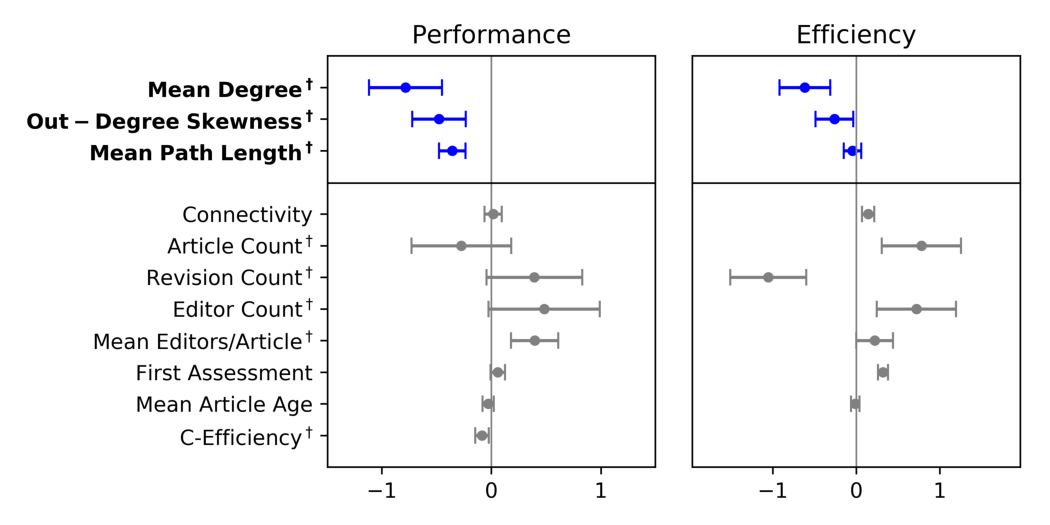
\includegraphics[scale=0.75]{regression.pdf}
\caption{
Regression coefficients for WikiProject success and coeditor network
properties
}
\end{center}
\end{figure}

\noindent[1] Giles, J. (2005). Internet encyclopaedias go head to head. {\em Nature.com}.
\\
\noindent[2] Keegan, B., \& Fiesler, C. (2017).
The Evolution and Consequences of Peer Producing Wikipedia’s Rules. In {\em ICWSM}.
\\
\noindent[3] Kearns, M. (2012). Experiments in social computation.
{\em Communications of the ACM}, 55(10).
\\
\noindent[4] Mason, W. A., Jones, A., \& Goldstone, R. L. (2008). Propagation of innovations in networked groups.
{\em Journal of Experimental Psychology: General}, 137(3).


% Place the abstract of your talk/poster here, 250 Words maximum.
% Mathematical formulae may be set in LaTeX, but do NOT use the
% bibliography environment -- if you must have references, use an 
% enumerated list.
%
% Your abstract (plus one figure) should not exceed one page.
%
% Check carefully.

%************************************
\end{document}